\documentclass[11pt]{report}
\usepackage[utf8]{inputenc}
\usepackage[a4paper, margin=1in]{geometry}
\usepackage{graphicx, color}
\usepackage{booktabs}
\usepackage[toc,page]{appendix}
\usepackage{pdfpages}
\usepackage{multicol}
\usepackage{changepage}
\usepackage{float}
\usepackage{multirow}
\usepackage{amsmath}
\usepackage[encoding,filenameencoding=utf8]{grffile}
\usepackage{subcaption}
\usepackage{csquotes}
\usepackage{hyperref, bookmark}

\setlength{\columnseprule}{0.5pt}
\def\columnseprulecolor{\color{black}}


% Package de algoritmos
\usepackage[portuguese,ruled,lined]{algorithm2e}

% Portuguese Encoding 
\usepackage[portuguese]{babel}
\usepackage[T1]{fontenc}

% import Java
\usepackage{listings} 

% Header
\usepackage{fancyhdr}
\pagestyle{fancy}
	\fancyhf{}
		\lhead{LEIC - ISEL}
    \rhead{Segurança Informática}

% Footer
\renewcommand{\headrulewidth}{1pt}
\renewcommand{\footrulewidth}{1pt}
\fancyfoot[CE,CO]{\thepage}


%%%%%%%%%%%%%%%%%%%%%%%%%%%%%%%%%%%%%%%%% CHANGES %%%%%%%%%%%%%%%%%%%%%%%%%%%%%%%%%


% Redefine the plain page style
\fancypagestyle{plain}{
\pagestyle{fancy}
  \fancyhf{}
	\lhead{LEIC - ISEL}
	\rhead{Segurança Informática}
	\renewcommand{\headrulewidth}{1pt}
	\renewcommand{\footrulewidth}{1pt}
\fancyfoot[CE,CO]{\thepage}
}

%%%%%%%%%%%%%%%%%%%%%%%%%%%%%%%%%%%%%%%%% CHANGES %%%%%%%%%%%%%%%%%%%%%%%%%%%%%%%%%

% Titulo e informação de capa
\title{Primeira Serie de exercícios}
\date{Outubro 2019}

% Define Chapter heading
\makeatletter
\def\@makechapterhead#1{%
  \vspace*{20\p@}%                                 % Insert 50pt (vertical) space
  {\parindent \z@ \raggedright \normalfont         % No paragraph indent, ragged right
%    \interlinepenalty\@M                           % Penalty
    \huge \bfseries #1\par\nobreak                 % Huge, bold chapter title
    \vskip 10\p@                                   % Insert 40pt (vertical) space
  }}
  
  %%%%%%%%%%%%%%%%%%%%%%%%%%%%%%%%%%%%%%%%% CHANGES %%%%%%%%%%%%%%%%%%%%%%%%%%%%%%%%%

\makeatother

%Custom commands

\renewcommand\appendixpagename{Anexos}
\renewcommand\appendixname{Anexo}
\renewcommand\appendixtocname{Anexos}

\newenvironment{subs}
  {\adjustwidth{2.5em}{0pt}}
  {\endadjustwidth}


% Retira a indentação ao início dos parágrafos 
\setlength{\parindent}{0em}
\newcommand{\blank}[1]{\hspace*{#1}\linebreak[0]}

% Section and Subsection spacing:
\usepackage{titlesec}
\usepackage{lipsum}



%%%%%%%%%%%%%%%%%%%%%%%%%%%%%%%%%%	DOCUMENT BEGINS	%%%%%%%%%%%%%%%%%%%%%%%%%%%%%%%%%%%%%

\begin{document}

%%%%%%%%%%%%%%%%%%%%%%%%%%%%%%%%%%%%%%%%%%%%%%%%%%%%%%%%%%%%%%%%%%%%%%%%%%%%%%%%%%%%%%%%%
%										COVER											%
%%%%%%%%%%%%%%%%%%%%%%%%%%%%%%%%%%%%%%%%%%%%%%%%%%%%%%%%%%%%%%%%%%%%%%%%%%%%%%%%%%%%%%%%%

\begin{titlepage} 

\newcommand{\HRule}{\rule{\linewidth}{0.5mm}} % Defines a new command for the horizontal lines, change thickness here

%----------------------------------------------------------------------------------------
%	LOGO SECTION
%----------------------------------------------------------------------------------------


\includegraphics[width=130pt, keepaspectratio=true]{img/logo_isel}\\[1cm] % Include a department/university logo - this will require the graphicx package
\center % Center everything on the page
 
%----------------------------------------------------------------------------------------
%	HEADING SECTIONS
%----------------------------------------------------------------------------------------

\textsc{\LARGE INSTITUTO SUPERIOR DE ENGENHARIA DE LISBOA}\\[1.5cm] % Name of your university/college
\vskip 40pt
\textsc{\Large SEGURANÇA INFORMÁTICA}\\[0.5cm] % Major heading such as course name
\textsc{\large LICENCIATURA ENGENHARIA INFORMÁTICA E COMPUTADORES}\\[0.5cm] % Minor heading such as course title
\vskip 40pt

%----------------------------------------------------------------------------------------
%	TITLE SECTION
%----------------------------------------------------------------------------------------

\HRule \\[0.4cm]
{ \LARGE \bfseries FASE DE EXERCÍCIOS }\\[0.4cm]
{ \huge \bfseries Fase 1}\\[0.4cm] % Title of your document
\HRule \\[1.5cm]
 
%----------------------------------------------------------------------------------------
%	AUTHOR SECTION
%----------------------------------------------------------------------------------------
\vskip 70pt
\begin{minipage}{0.4\textwidth}
\begin{flushleft} \large
\emph{Autores:}\\
43552 - Samuel \textsc{Costa}\\
43320 - André \textsc{Mendes}
\end{flushleft}
\end{minipage}
~
\begin{minipage}{0.4\textwidth}
\begin{flushright} \large
\emph{Docente:} \\
José \textsc{Simão}\\
\end{flushright}
\end{minipage}\\[3cm]

%----------------------------------------------------------------------------------------
%	DATE SECTION
%----------------------------------------------------------------------------------------

{\large 21 de Outubro de 2019}\\[3cm] % Date, change the \today to a set date if you want to be precise

%----------------------------------------------------------------------------------------

\vfill % Fill the rest of the page with whitespace

\end{titlepage}


\renewcommand\thesection{\arabic{section}}

\pdfbookmark{\contentsname}{toc}
\tableofcontents


\newpage


\section{Introdução}
O trabalho realizado para este fase pretende que os temas desenvolvidos durante as aulas sejam postos em prática. Para esta fase os exercícios focaram essencialmente a primeira parte da matéria.\\

\begin{itemize}
  \item Esquemas e Primitivas Criptográficas
  \item Java Cryptographic Architecture (JCA)
  \item Certificados digitais e Infraestrutura de Chave Pública
  \item Protocolo Criptográfico Transport Layer Security (SSL/TLS)
\end{itemize}

Neste trabalho prático pretendemos responder aos vários exercícios propostos e implementar uma demonstração dos pontos referidos.

\newpage

\section{Primeira série de exercícios}
\subsection{Exercício 1}

Ambos os esquemas criptográficos visam garantir a autenticidade da mensagem adicionando à própria mensagem um numero de bits de forma a identificar o emissor da mesma, no caso do MAC uma marca ou uma assinatura no caso da assinatura digital, sendo essa autenticidade verificada no recetor. Ambos os esquemas utilizam chaves privadas para "marcar" \space a mensagem, sendo que no caso da assinatura digital é usado uma chave publica para autenticar essa mesma mensagem, já no esquema MAC é usada uma chave simétrica.\\

\subsection{Exercício 2}
A organização da função de hash reduz uma mensagem de tamanho variável $ m $ a um bloco de tamanho $ n $ ou seja, a dimensão de $ yL = $ dimensão de $ m1 $, logo $ n $ bits $ = $ dimensão de um bloco <<<\space dimensão da mensagem, pelo que existe $ m $ e $ m' $, tal que $ H(m) = H(m')$. O diagrama seguinte pretende ilustrar a organização da aplicação da primitiva de cifra, conforme explicitado:\\

\begin{figure}[H]
	\centering
	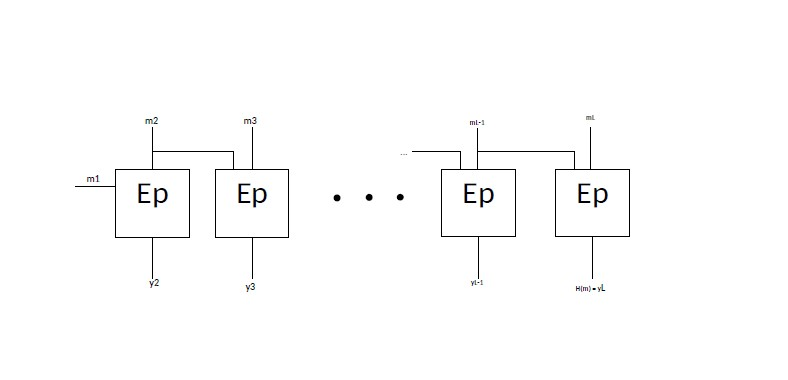
\includegraphics[scale=0.5]{img/ex2.jpg}
	\caption{Exemplo da cifra}
\end{figure}

\subsection{Exercício 3}
Apesar de não ter acesso ao texto em claro, o que facilitaria o ataque, o atacante tem acesso ao texto cifrado. Sabendo que os mesmos blocos de texto em claro produzem as mesmas cifras, então um oráculo de encriptação pode ser usado. Se o atacante pode submeter texto em claro para encriptação, então também pode verificar hipóteses sobre o texto em claro que corresponde ao texto cifrado.\\

\newpage

\subsection{Exercício 4}
Comparando os dois esquemas seria expectável que a primitiva AES fosse em todos os casos mais dificil de criptoanalizar que um sistema com primitiva DES, no entanto essa analise tem de ser feita também relativamente ao modo de operação que cada uma pode usar, como por exemplo no caso especifico de um sistema AES ter usado um modo de operação ECB (Electronic Code Book) e a sua mensagem ser de alguma forma curta e padronizada pode mais facilmente ser quebrada que uma DES que usou o mode de operação CBC (Cipher Block Chain).\\

\subsection{Exercício 5}
A JCA contem uma arquitectura baseada em providers e uma série de APIs para assinaturas digitais, hashes, certificados e a sua validação, encriptação, geração e gestão de chaves. Essas APIs permitem integrar segurança facilmente no código.
Uma engine class fornece a interface para um serviço criptográfico especifico, ficando independente de um algoritmo criptografico particular ou de um provider. As engine classes fornecem operações criptograficas ou geradores ou conversores de material criptografico, ou objectos que encapsulam dados criptograficos e podem ser usados em niveis mais elevados de abstração.
Esta opção de arquitectura privilegia a independencia de implementação e a interoperabilidade, já que as aplicações não precisam de implementar algoritmos de segurança e os providers são interoperáveis em relação às aplicações.\\

\subsection{Exercício 6.1}
Um certificado é composto pelo seu corpo (campos, extensões e propriedades) e por uma assinatura. A verificação da assinatura permite atestar da autenticidade da mensagem.
Como o processo de verificação da autenticidade calcula um hash do corpo do certificado, não deve ser possível que mensagens diferentes produzam o mesmo hash (2ª pré-imagem), o que significaria que um certificado podia ser alterado no seu corpo ( por exemplo, no seu emissor ou chave pública) e a verificação da assinatura retornar true.\\

\subsection{Exercício 6.2}
Para validar a assinatura do certificado C são usados o seu corpo, a assinatura presentes no certificado e a chave pública do emissor. Para validar os outros certificados intermédios na cadeia de certificação são usados os mesmos elementos. Para validar a assinatura do certificado raíz, é usada a sua chave pública, uma vez que nesse caso o certificado é assinado pelo emissor (auto-assinado). Portanto, nenhuma chave privada é usada para na validação de certificados X.509.\\

\subsection{Exercício 7}
Para este exercício foram realizadas experiências segundo o \textit{Labs for Security Eduction}.\\
Na alnea 1 do ponto \emph{"2.4 Task 4: Padding"} foram testadas os modos propostos e é possivel concluir que ECB e CBF, ambos usam \textit{padding}, ao contrário dos modos CFB e OFB.\\
Para determinar o uso de \textit{padding} nos varios modos foi usado um ficheiro de 5 \textit{bytes} e depois foi feita a sua decifra usando o comando \textit{nopad} e também um \textit{hexdump} para verificar o seu conteúdo. Foi também possível verificar que o tamanho do ficheiro no caso dos modos que usam \textit{padding} era sempre uma potência de base 2.\\

Na alínea 2 exercício usando a \textit{-aes-128-cbc} para encriptar os 3 ficheiros propostos foi possível reparar que os ficheiros todos os ficheiros tiveram \textit{padding}. O de 5 e o de 10 \textit{bytes} tiveram um preenchimento de \textit{padding} até aos 16  \textit{bytes}, sendo que o de 16 ao ser cifrado obtinha o seu preenchimento completo então levou mais 16 \textit{bytes} de \textit{padding}.\\ 
Os valores de preenchimento pode ser verificados com o \textit{hexdump} dos três ficheiros.

\begin{figure}[H]
	\centering
	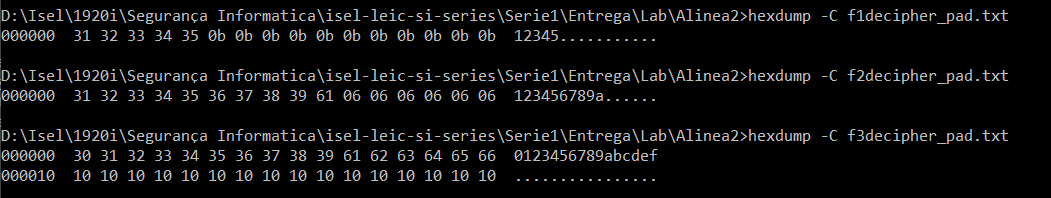
\includegraphics[scale=0.5]{img/padding}
	\caption{hexdump on files}
\end{figure}

\subsection{Exercício 8.1}
A função de decifra e verificação é dada por: T(k2)(D(k1)(c)||t). Ou seja, aplicando a primitiva de decifra ao criptograma, e de seguida verificando a assinatura contra a mensagem e a marca.\\

\subsection{Exercício 8.2}
Foi implementada a aplicação Mac-then-encrypt usando a JCA.\\

\subsection{Exercício 9}
Implementação em código \\
\newpage


\end{document}
